\begin{enumerate}
	\item
	\begin{enumerate}
		\item $4 \longrightarrow 4+3=7 \longrightarrow 7^{2}=49 \longrightarrow 49-9=40$.

		On obtient bien 40 avec le programme A avec 4 comme nombre de départ.

		\item $4 \longrightarrow 4+6=10 \longrightarrow 10\times 4=40$.

		On obtient 40 avec le programme B avec 4 comme nombre de départ.
	\end{enumerate}

	\item On saisit en B3 la formule \texttt{=(B1+6)*B1}.

	\item~
	
	\begin{center}
	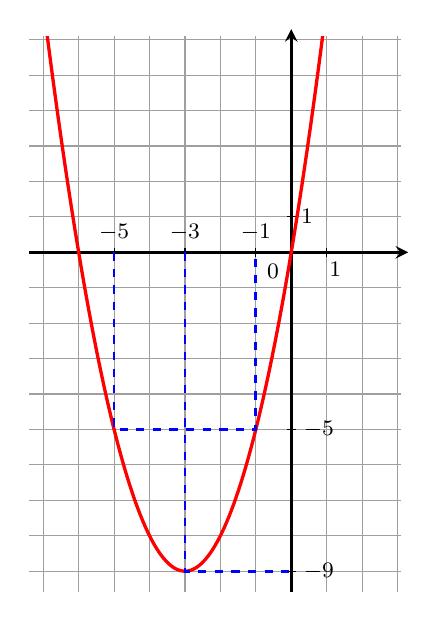
\begin{tikzpicture}[scale=0.45,>=stealth]
		\draw[gray!75,line width=0.4pt] (-7.4,-9.6) grid (3.1,6.1);
		\draw[->,line width=1pt] (-7.4,0) -- (3.3,0);
		\draw[->,line width=1pt] (0,-9.6) -- (0,6.3);
		\draw (1,-0.12) -- (1,0.12); \node[below right] at (0.8,0) {\footnotesize 1};
		\draw (-0.12,1) -- (0.12,1); \node[right] at (0,1) {\footnotesize 1};
		\draw (-2pt,-2pt) node[below left] {\footnotesize 0};
		% --- graduations négatives sur l'axe des abscisses ---
		\draw (-1,-0.12) -- (-1,0.12);
		\node[above] at (-1,0.05) {\footnotesize $-1$};
		\draw (-3,-0.12) -- (-3,0.12); \node[above] at (-3,0.05) {\footnotesize $-3$};
		\draw (-5,-0.12) -- (-5,0.12); \node[above] at (-5,0.05) {\footnotesize $-5$};
		% --- graduations négatives sur l'axe des ordonnées ---
		\draw (-0.12,-5) -- (0.12,-5); \node[right] at (0.08,-5) {\footnotesize $-5$};
		\draw (-0.12,-9) -- (0.12,-9); \node[right] at (0.08,-9) {\footnotesize $-9$};
		\begin{scope}
			\clip (-7.4,-9.6) rectangle (3.1,6.1);
			\draw[red,line width=1.2pt,domain=-7.2:0.9,samples=120] plot (\x,{\x*\x+6*\x});
		\end{scope}
		\draw[blue,dashed,line width=1pt] (-3,0) -- (-3,-9) -- (0,-9);
		\draw[blue,dashed,line width=1pt] (-5,0) -- (-5,-5) -- (-1,-5) -- (-1,0);
	\end{tikzpicture}
\end{center}
	\begin{enumerate}
		\item Par lecture graphique, l'image de $-3$ par la fonction $f$ est $-9$.

		\item Par lecture graphique, les antécédents de $-5$ par la fonction $f$ sont $-5$ et $-1$.
	\end{enumerate}

	\item En choisissant $x$ comme nombre de départ dans le programme B, le résultat est $x(x+6)$.
	
	Or, un produit est nul si et seulement si l'un au moins de ses facteurs est nul :
	\[x(x+6)=0 \iff x=0 \ \text{ ou } \ x+6=0 \iff x=0 \ \text{ ou } \ x=-6.\]
	Les nombres qui permettent d'obtenir 0 par le programme B sont 0 et $-6$.

	\item
	\begin{enumerate}
		\item $(x+3)(x+3)=x\times x+x\times 3+3\times x+3\times 3=x^{2}+3x+3x+9=x^{2}+6x+9$.

		\item Avec le programme A, on obtient $(x+3)^{2}-9=x^{2}+6x+9-9=x^{2}+6x$.

		Avec le programme B, on obtient $(x+6)\times x=x^{2}+6x$.

		Les deux programmes donnent le même résultat quel que soit le nombre $x$ choisi au départ.
	\end{enumerate}
\end{enumerate}
